\documentclass{article}
\usepackage[utf8]{inputenc}
\usepackage{ebgaramond}
\usepackage[czech]{babel}
\usepackage{csquotes}
\usepackage[T1]{fontenc}
\usepackage{makecell}
\usepackage{float}
\usepackage{graphicx}
\graphicspath{ {./images/} }

\usepackage[
backend=biber,
style=ieee
]{biblatex}

\addbibresource{biblio.bib}

\begin{document}

\begin{titlepage}
    \begin{center}
        \huge \textsc{Vysoké učení technické v~Brně\\
        \huge Fakulta informačních technologií}\\
        \vspace{\stretch{0.382}}
        \LARGE Modelování a simulace\,--\,simulační studie\\
        \Huge Studie morfologie kolonie hub pomocí celulárního automatu\\
        \vspace{\stretch{0.618}}
    \end{center}
    \Large \hfill Hung Do (xdohun00) \\
    {\Large \today \hfill Marek Dohnal (xdohna48)}
\end{titlepage}

\tableofcontents
\newpage

\section{Procesy v koloniích hub}
V koloniích hub můžeme nalézt mnoho komplexních biologických procesů, které vykazují různé charakteristiky, lišící se napříč rozmanitými druhy v říší Fungi. Mezi nejznámější z nich patří například fermentace, která se využívá například pro zvýšení trvanlivosti potravin. Mezi příčiny rozdílů mezi procesy napříč různými druhy hub lze řadit způsob, jakým se houba rozmnožuje (sexuálně, asexuálně), nebo metodu příjmu potravy (symbioticky, parazitně, saprofiticky). 

Naše studie se soustředí na užší skupinu těchto procesů. Zaměřujeme se na kolonii hub, rostoucí na zdroji živin, který konzumuje, a se kterým dále neinteraguje. Důsledkem konzumace živin se může kolonie nepohlavně rozmnožovat dělením jedinců, biomasa se takto rozrůstá a následkem toho ubývá živin z prostředí. Morfologie, hustota a velikost výsledné kolonie se liší z velké části na základě množství živin, které prostředí poskytuje. Substrát, obsahující nižší počet živin, vede k řidší kolonii, ve které se vyskytuje viditelné větvení. Prostředí s vysokou koncentrací živin naopak produkuje kolonie uniformní a husté biomasy \cite{solidSubstrates} \cite{morphological}. 

Charakteristika růstu kolonií hub byla předmětem dvou studií, které k modelování přistupují různými způsoby. První studie předkládá několik modelů založených na celulárních automatech s různě složitými tranzitivními funkcemi, avšak neexperimentuje s různým množstvím živin v prostředí \cite{solidSubstrates}. 
Druhá studie se blíže zaměřuje na morfologii kolonie, a simuluje její vývoj pomocí komplexnějšího matematického modelu, využívajícího diferenciálních rovnic. Výstupem je více či méně členitá vrstevnice, která "roste" z počáteční úsečky spor. \cite{morphological}

Cílem naší studie je zjistit, zda lze upravit některý z modelů navržen Josephem Laszlem a Robertem Silmanem \cite{solidSubstrates} tak, aby se v simulaci projevily morfologické změny kolonie závisející na rozdílném množství živin v prostředí.

\section{Návrh modelu kolonie}

Návrh modelu si vyžaduje abstrakci skutečného systému reprodukce hub a jejich interakce s prostředím. Míra abstrakce, kterou volíme, je poměrně vysoká.  Neimplementujeme existující komplexní matematické modely, které počítají například s vlivem živin na toxicitu prostředí \cite{toxicMetals}, a jsou schopny lépe reflektovat více vnějších vlivů na růst kolonie. Náš model v kontrastu pracuje pouze s jedním vlivem, kterým je množství živin v prostředí. Zároveň náš model nepracuje v definovaném časovém a prostorovém měřítku; jelikož naším cílem je studovat pouze morfologii kolonie, nezabýváme se modelováním dosažené velikosti kolonie v určitém čase. Reprezentace rozmnožování v automatu se liší od skutečnosti v tom, že spory se v modelu rozmnožují pouze fragmentací podhoubí do nejbližšího 8-okolí, ale ve skutečnosti kromě tohoto procesu také dochází k disperzi spor do větších vzdáleností. 

Prostředí, ve kterém kolonie roste, konceptualizujeme jako čtvercové pole buněk celulárního automatu, které samo o sobě neuchovává žádné hodnoty. Každá buňka spravuje svůj stav, a veškeré změny v systému jsou modelovány změnami stavů buněk.

Návrh pravidel automatu se zakládá na dvou předpokladech: nižší množství živin má za důsledek řidší a méně uniformní kolonii, která má větší sklony k větvení \cite{solidSubstrates} \cite{morphological}, a zároveň způsobuje diferenciaci mezi buňkami kolonie \cite{differentiation}. 

Proces, kterým si každá buňka projde je rozdělen do několika fází, přičemž většina přechodů mezi fázemi je implementována jako stochastický proces, viz. tabulka \ref{model2ext_cellaging_table}. Buňka začíná v prázdném stavu, který modeluje absenci biomasy. Pokud je v jejím prostředí určité množství neprázdných buněk, t. j. buněk reprezentujících houbovou tkáň, buňka se stane vegetativní houbovou tkání. Dále takto obsazená buňka podléhá třem fázím stárnutí, každá fáze sestává ze 4 stochastických kroků v automatu. Nejprve na vegetativním podhoubí dochází k vývoji tzv. "foot cells", které jsou počáteční fází dospívání kolonie. Následně dochází k vývoji konidiofor, které jsou nosičem struktur sloužících k reprodukci. Konečná fáze je dospělost těchto struktur, ze kterých se u skutečných kolonií šíří spory \cite{differentiation}. Pokud prázdná buňka není obsazena dochází k úbytku živin. Tento proces je modelován jako 4 stochastické kroky automatu, po kterých se buňka stane nedostupnou pro obsazení následkem reprodukce. 

Náš model se dá chápat jako rozšířené spojení Modelu 1a, Modelu 2a a Modelu 4 Josepha Laszla a Roberta Silmana \cite{solidSubstrates}.
Z Modelu 1a jsme převzali pravidla pro dělení buňek, proces konzumace živin jsme implementovali na základě Modelu 2a, a Model 4 jsme rozšířili o další stav, a následně implementovali jako reprezentaci stárnutí kolonie. 
V tabulce \ref{model2ext_cellaging_table} je popsána výsledná množina pravidel nově navrženého automatu.


\section{Implementace modelu}
Naši simulaci jsme napsali v jazyku \verb|C| za použití knihovny \verb|ncurses|. Soubory jsou rozděleny do dvou složek: ve složce \verb|./include| nalezneme hlavičkové soubory a v \verb|./src| zdrojové soubory. V programu se nachází dvě dvourozměrná pole o velikosti \verb|400x200| buněk udržující stav v dané buňky. Jedno pole slouží ke čtení a zobrazení (\uv{front buffer}) a druhý slouží na zápis další iterace (\uv{back buffer}). Po dokončení iterace se tyto dvě pole prohodí (\uv{back} se zobrazí a \uv{front} je připraveno na zápis).

Program začíná v hlavní funkci, ve které se volají inicializační a nastavovací funkce společně s načítáním argumentů. Poté se spouští nekonečný cyklus programu, ve kterém se zpracovávají uživatelské vstupy, aktualizace a zobrazení stavu celulárního automatu.

Soubor \verb|./include/board.h| deklaruje rozhraní pro práci se samotným automatem. Nejdůležitějšími funkcemi rozhraní je funkce \verb|void apply_rules(struct board_t *)|, skrz který může programátor definovat chování/pravidla automatu. Ta jsou definována v modulech \verb|board_rule1.c|, \verb|board_rule2.c| a \verb|board_rule_aging|.

Nakonec se zde nachází soubory \verb|./include/board_setup.h| a \verb|./src/board_setup.c| definující počáteční pozici celulárního automatu. Soubor \verb|.c| je vygenerovaný pomocí přiloženého Python skriptu \verb|pixel_editor.py|.

Program byl testován primárně na systému \verb|Linux 5.15-78-1-MANJARO x86_64 GNU/Linux|, nicméně se ho podařilo rozjet i na jiných systémech jako: 
\begin{itemize}
    \item \verb|FreeBSD 13.1-STABLE|
    \item \verb|Linux CentoOS 5.4.225 x86_64 GNU/Linux|
    \item \verb|Linux Ubuntu 20.04 LTS  5.10.102.1-microsoft-standard-WSL2 x86_64 GNU/Linux|
\end{itemize}

\section{Nastavená pravidla modelů automatu}

\subsection{Pravidla prvního modelu}

\begin{table}[H]
    \centering
    \begin{tabular}{|c|c|} \hline
        \multicolumn{2}{|c|}{\textbf{Prázdná buňka}}                    \\ \hline
        \thead{Počet okupovaných \\ sousedů} & \thead{Šance \\ na růst} \\ \hline
         1                          &  12.5 \%                          \\ \hline
         2-8                        &     0 \%                          \\ \hline
    \end{tabular}
    \caption{Tabulka s pravidly prvního modelu}
    \label{model1table}
\end{table}

\subsection{Pravidla druhého modelu}
\begin{table}[ht]
    \centering
    \begin{tabular}{|c|c|c|c|c|c|c|} \hline
        \multicolumn{7}{|c|}{\textbf{Prázdná buňka}} \\ \hline
        \thead{Počet \\ sousedů} & \thead{Šance na růst \\ \textbf{NH} -> 1-3} & \thead{Šance na růst \\ \textbf{NH} == 4} & \thead{Šance na růst \\ \textbf{NH} == 5 } & \thead{Šance na růst \\ \textbf{NH} -> 6-7} & \thead{Šance na růst \\ \textbf{NH} >= 8} & \thead{Šance na úbytek \\ živin v buňce} \\ \hline
                1   &  12.5 \%   &   12.5 \%   &   12.5 \%  &   12.5 \%  &  12.5 \%  &   50 \%   \\ \hline
                2   &     0 \%   &     25 \%   &     25 \%  &     25 \%  &    25 \%  &   75 \%   \\ \hline
                3   &     0 \%   &      0 \%   &     50 \%  &     50 \%  &    50 \%  &  100 \%   \\ \hline
                4   &     0 \%   &      0 \%   &      0 \%  &     50 \%  &    50 \%  &  100 \%   \\ \hline
                5   &     0 \%   &      0 \%   &      0 \%  &      0 \%  &    50 \%  &  100 \%   \\ \hline
               6-8  &     0 \%   &      0 \%   &      0 \%  &      0 \%  &     0 \%  &  100 \%   \\ \hline
    \end{tabular}
    \caption{Tabulka s pravidly druhého modelu}
    \label{model2table}
\end{table}

\subsection{Pravidla rozšířeného druhého modelu}

\begin{table}[ht]
    \centering    
    \begin{tabular}{|c|c|c|c|c|c|c|c|} \hline
        \multicolumn{7}{|c|}{\textbf{Prázdná buňka}} & \textbf{Živá buňka}\\ \hline
        \thead{Počet \\ sousedů} & \thead{Šance na růst \\ \textbf{NH} -> 1-3} & \thead{Šance na růst \\ \textbf{NH} == 4} & \thead{Šance na růst \\ \textbf{NH} == 5 } & \thead{Šance na růst \\ \textbf{NH} -> 6-7} & \thead{Šance na růst \\ \textbf{NH} >= 8} & \thead{Šance na úbytek \\ živin v buňce} & \thead{Šance na \\ stárnutí buňky} \\ \hline
                1   &  12.5 \%   &   12.5 \%   &   12.5 \%  &   12.5 \%  &  12.5 \%  &   50 \%  &      0 \% \\ \hline
                2   &     0 \%   &     25 \%   &     25 \%  &     25 \%  &    25 \%  &   75 \%  &      0 \% \\ \hline
                3   &     0 \%   &      0 \%   &     50 \%  &     50 \%  &    50 \%  &  100 \%  &   12.5 \% \\ \hline
                4   &     0 \%   &      0 \%   &      0 \%  &     50 \%  &    50 \%  &  100 \%  &   12.5 \% \\ \hline
                5   &     0 \%   &      0 \%   &      0 \%  &      0 \%  &    50 \%  &  100 \%  &   12.5 \% \\ \hline
               6-8  &     0 \%   &      0 \%   &      0 \%  &      0 \%  &     0 \%  &  100 \%  &   12.5 \% \\ \hline
    \end{tabular}
    \caption{Tabulka s pravidly rozšířeného modelu}
    \label{model2ext_cellaging_table}
\end{table}

\section{Chování modelu a simulace kolonie}
Pro demonstraci chování modelu jsme šestkrát simulaci přes 150 iterací s jinými nutričními parametry. Model akceptuje nutriční parametry v rozsahu 1 až nekonečno, ovšem experimentálně jsme zjistili, že se výsledky znatelně liší jen mezi úrovněmi 1 až 6. Nutriční parametry udávají, kolika fázemi se prochází při konzumaci živin buňky. Pro úroveň $n$ se projde $n + 1$ fázemi, než se buňka stane neobsaditelnou. Výsledky simulace jsou zobrazeny v obrázku
\ref{grid}

Výsledek c) byl spuštěn se stejnými parametry jako Model 4 studie \cite{solidSubstrates}. Náš výsledek se liší od původní implementace tím, že zde nedochází k tak výrazné diferenciaci kolonie. Tento rozdíl je dle nás způsoben nižším počtem iterací (150 iterací proti 275 iteracím původních autorů). Výsledek d) se výsledku Modelu 4 původních autorů blíží nejvíce.

Zbytek výsledků jsme porovnávali se studií \cite{morphological} z hlediska prostorové morfologie, a se studií \cite{differentiation} z hlediska morfologie diferenciační. Můžeme pozorovat, že simulace b) nejvíce aproximuje řídký růst podhoubí a nepravidelný rozmach kolonie patrný z obrázku obrázku 1d studie \cite{morphological}. Další simulace z hlediska prostorové morfologie konvergují směrem k hladším hranám a hustšímu růstu se zvyšujícím se množstvím živin, stejně jako ve studii \cite{morphological}. U simulace a) můžeme pozorovat velice malý prostorový rozmach.

Reprezentaci diferenciační morfologie lze vidět nejlépe na simulacích d), e) a f). Na všech třech výsledcích jsou patrné barevné koncentrické kruhy, které reprezentují zóny stárnutí. Je zde vidět, že větší množství živin má za následek větší míru diferenciace. \cite{differentiation} Stárnutí je málo patrné u modelů a), b), a c).

V tabulce \ref{results} jsou statistiky jednotlivých studií. Smyslem těchto statistik je dát do souvislosti počet houbových buňek a neobyvatelných buněk. Můžeme pozorovat, že u simulací a) až d) počet neobyvatelných buněk vůči simulacím s menším nutričním parametrem narůstá a ovlivňuje výslednou morfologii kolonie. U výsledků e) a f) naopak klesá a již není příliš podstatným faktorem pro výsledný tvar kolonie. 

\begin{table}[ht]
    \centering    
    \begin{tabular}{|c|c|c|c|c|} \hline
        \thead{Výsledek} & \thead{Nutriční \\ parametr} & \thead{Počet \\ živých buňěk} & \thead{Počet \\ neobyvatelných buňek} & \thead{Poměr \\ živých buňek k \\ neobyvatelným buňkám} \\ \hline
                a)   & 1   &  89  &   229   &   0,3886 \\ \hline
                b)  & 2   &  1664  &   3165   &   0,5258 \\ \hline
                c)  & 3   &  2957  &   5144   &   0,5748 \\ \hline
                d)   & 4   &  8466  &   7518   &   1,1167 \\ \hline
                e)  & 5   &  14582  &   6172   &   2,3496 \\ \hline
                f)   & 6   &  18925  &   4488   &   4,2933 \\ \hline
    \end{tabular}
    \caption{Tabulka se statistikami jednotlivých výsledků}
    \label{results}
\end{table}



\clearpage
\begin{figure}[ht]
\centering
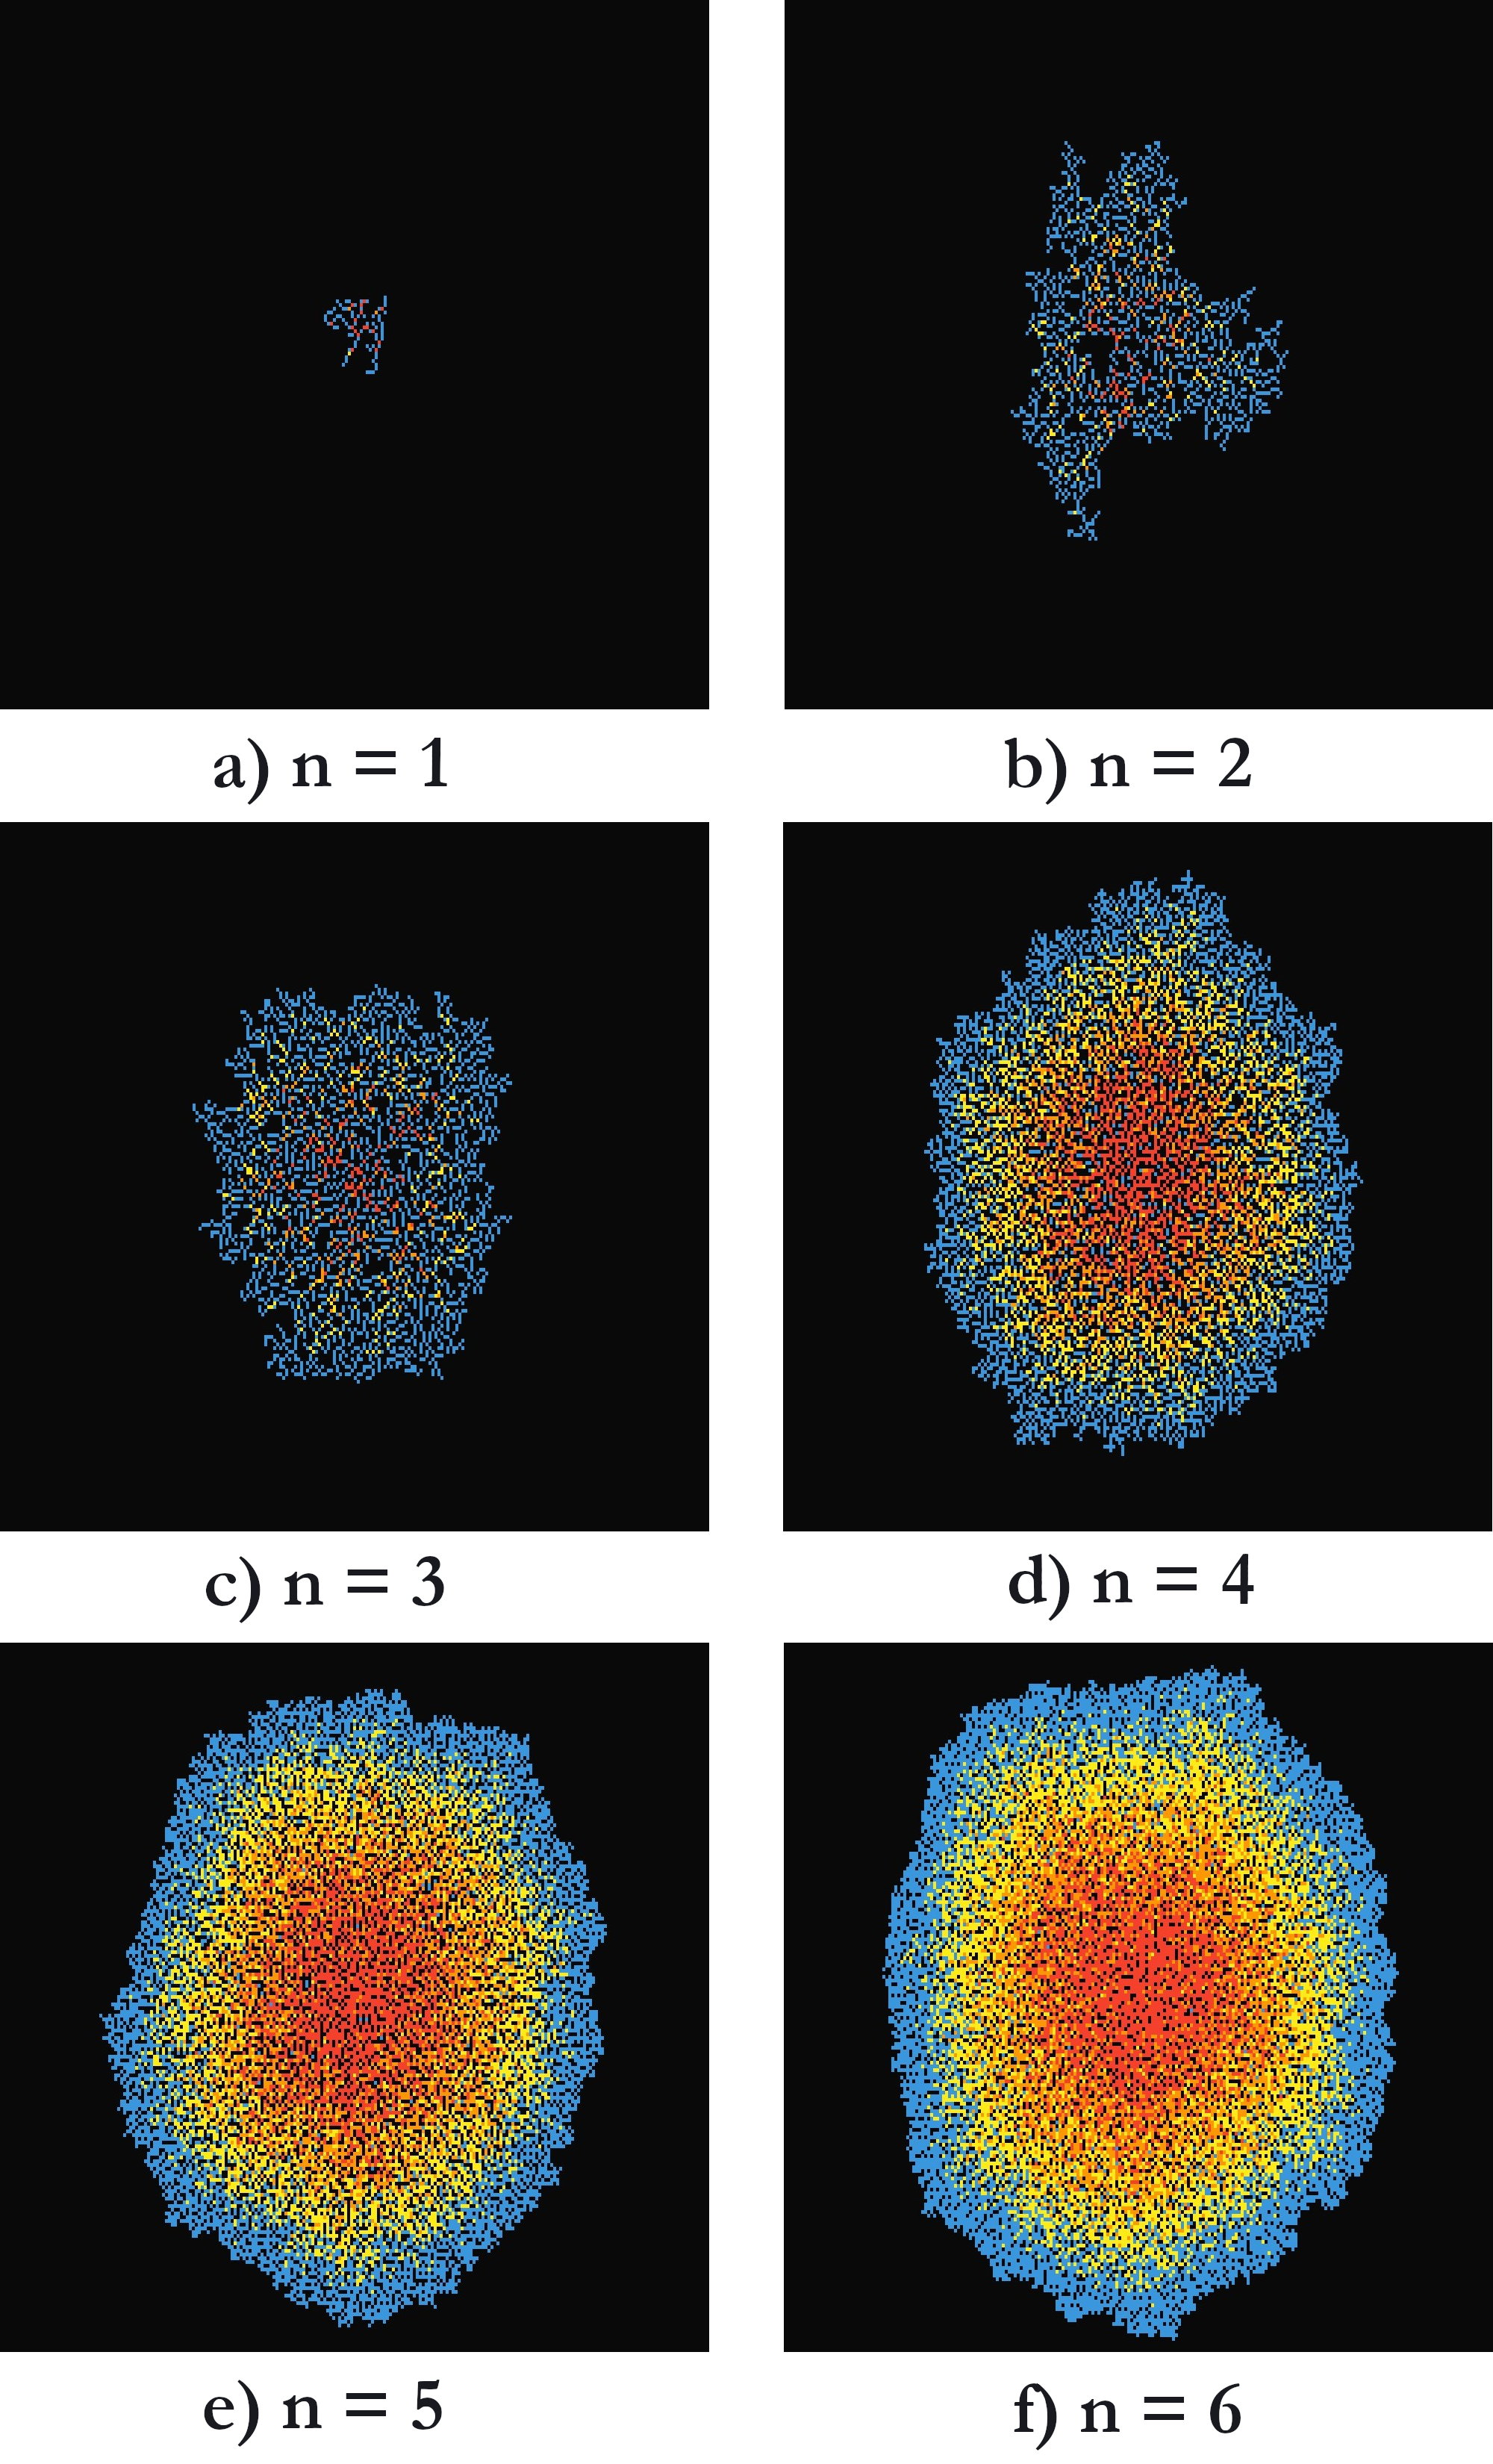
\includegraphics[width=0.95\textwidth]{grid.jpg}
\caption{Výsledky modelu pro počáteční nutriční hodnoty 1 až 6, a 150 iterací.}
\label{grid}
\end{figure}
\clearpage

\section{Závěr a zhodnocení modelu}
Výsledné simulace ukázaly, že model je schopen přibližně reflektovat morfologické změny způsobené změnou živin. Jako přednost modelu by se dala vyzdvihnout jeho jednoduchost. Narozdíl od komplexních matematických modelů lze pravidla našeho celulárního automatu shrnout do tabulky, a snáze je pochopit. Model na druhou stranu nevykazuje velkou flexibilitu. Experimentálně se ukázalo, že model dokáže reflektovat výraznější změny pro zhruba 4 různé nutriční hladiny. Z hlediska prostorové morfologie potom dochází k přílišnému zmenšování kolonie u simulací a) a b) v porovnání se studií \cite{morphological}. Prostorová diferenciace je znázorněna nejlépe u simulací s vyšším nutričním parametrem. Jsou zde dobře viditelné kruhy, které kolonii rozdělují do vývojových fází. V simulacích s nízkým množstvím živin naopak k přílišné diferenciaci nedochází, protože ji malé množství živin nedovoluje \cite{differentiation}. 

Konstatujeme, že model je schopen reflektovat dopad živin na prostorovou charakteristiku a stárnutí kolonie. Model by se dalo vylepšit například tak, že by v příští variantě implementovalo pravidlo, které by mělo za následek větší prostorové šíření kolonie při nízkých nutričních hodnotách. 
\printbibliography

\end{document}
